You can open the search dialog (\bxfigref{SearchDialog}) from the toolbar, by pressing \bxkey{Ctrl+H} or via the menu:\\
\bxmenu{Search}{Search}{}\\

\begin{figure}[h]
\begin{center}
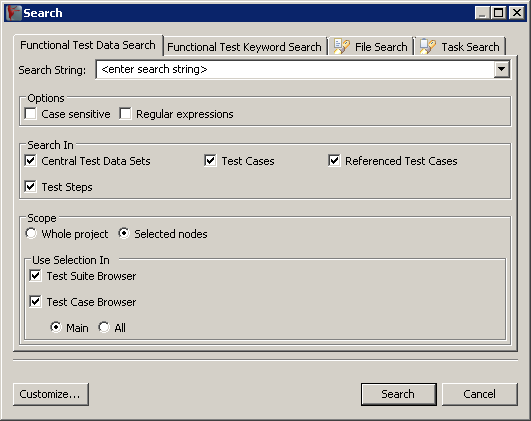
\includegraphics[width=0.50\textwidth]{Tasks/Searching/PS/SearchDialog}
\caption{Search Dialog}
\label{SearchDialog}
\end{center}
\end{figure}

The search dialog allows you to search the \textbf{current \gdproject{} in the  current working language} for:

\begin{itemize}
\item Keywords \bxpref{TasksSearchKeywords} (\gdcases{}, \gdsteps{}, \gdsuites{}, \gdjobs{} and categories).
\item Test data used in \gdcases{} or central test data sets \bxpref{TasksSearchData}.
\item Files in the workspace \bxpref{TasksSearchFiles}.
%\item Tasks in the repository \bxpref{TasksSearchTasks}.
\end{itemize}


\subsubsection{Searching for keywords (\gdcases{}, \gdsteps{}, \gdsuites{}, \gdjobs{} and categories) throughout the \gdproject{}}
\gdhelpid{testSpecificationViewContextId}{Test Case Browser}
\gdhelpid{testExecViewContextId}{Test Suite Browser}
\gdhelpid{com.bredexsw.guidancer.doc.keywordSearchPageContextId}{Keyword Search}
\label{TasksSearchKeywords}

On the first tab of the search dialog, you can search for the following based on their name:

\begin{itemize}
\item \gdsteps{}
\item \gdcases{} -- either the original specification or places where a \gdcase{} has been reused (referenced)
\item \gdsuites{} -- either the original specification or places where a \gdsuite{} has been reused (referenced)
\item \gdjobs{}
\item Categories
\end{itemize}

Enter the term you wish to search for and select whether you want the search term to be case sensitive or whether you will be using regular expressions. You can also specify whether you want to search in the whole \gdproject{}, or just for the selected nodes \bxpref{TasksSearchLimit}.

Click \bxcaption{Search} to start the search. The results are shown in the \gdsearchresultview{} \bxpref{TasksSearchResultView}. 

\bxtipp{Only names from within the current \gdproject{} and in the current working language are displayed. Names from reused \gdprojects{} are not found.}

\subsubsection{Searching for test data}
\gdhelpid{testSpecificationViewContextId}{Test Case Browser}
\gdhelpid{testExecViewContextId}{Test Suite Browser}
\gdhelpid{com.bredexsw.guidancer.doc.testDataSearchPageContextId}{Test Data Search}
\label{TasksSearchData}

On the second tab of the search dialog, you can search for test data in the following:

\begin{itemize}
\item Central test data sets
\item \gdcases{} -- either either the original specification or places where a \gdcase{} has been reused (referenced)
\item \gdsteps{}
\end{itemize}

\bxtipp{The search does not consider the \bxname{name} of the central test data set, for example, only the data contained in it.}

Enter the term you wish to search for and select whether you want the search term to be case sensitive or whether you will be using regular expressions. You can also specify whether you want to search in the whole \gdproject{}, or just for the selected nodes \bxpref{TasksSearchLimit}.

Click \bxcaption{Search} to start the search. The results are shown in the \gdsearchresultview{} \bxpref{TasksSearchResultView}. 

\bxtipp{Only test data from within the current \gdproject{} and in the current working language is displayed. Data from reused \gdprojects{} is not found.}

\subsubsection{Searching for files in the workspace}
\gdhelpid{testSpecificationViewContextId}{Test Case Browser}
\gdhelpid{testExecViewContextId}{Test Suite Browser}
\label{TasksSearchFiles}

On the third tab of the search dialog, you can search for and in files contained in your workspace.

Enter the term you wish to search for and click \bxcaption{Search} to start the search. The results are shown in the \gdsearchresultview{} \bxpref{TasksSearchResultView}. 

\subsubsection{Limiting the search to the selected node}
\gdhelpid{com.bredexsw.guidancer.doc.keywordSearchPageContextId}{Keyword Search}
\gdhelpid{com.bredexsw.guidancer.doc.testDataSearchPageContextId}{Test Data Search}
\label{TasksSearchLimit}

In the search dialog, you can specify whether the search you define should be performed on the whole \gdproject{}, or just on the node you have selected in a browser. If you select to just search within the selected node, then you can define which browser or browsers to search in (you may have more than one active selection in your browsers):

\begin{description}
\item [\gdtestsuitebrowser{}]{This search will be limited to the selected item (\gdsuite{}, \gdjob{}, category) in the \gdtestsuitebrowser{}. If you select the root node in the \gdtestsuitebrowser{}, then the whole \gdtestsuitebrowser{} will be searched. }
\item [Main \gdtestcasebrowser{}]{This search will be limited to the selected item (\gdcase{}, category) in the \gdtestcasebrowser{}. If you have more than one \gdtestcasebrowser{} open \bxpref{TasksMultipleTCB}, then the one marked as \bxname{Main} will be used. If you select the root node in the \gdtestcasebrowser{}, then the whole \gdtestcasebrowser{} will be searched.}
\item [All Test Case Browsers]{If you have more than one \gdtestcasebrowser{} open \bxpref{TasksMultipleTCB}, then the selected nodes in all of them will be searched.If you select the root node in the \gdtestcasebrowser{}, then the whole \gdtestcasebrowser{} will be searched.  }
\end{description}

You can select one or more of these options to perform the search. 

%% \subsubsection{Searching for tasks in Mylyn}
%% \gdhelpid{testSpecificationViewContextId}{Test Case Browser}
%% \gdhelpid{testExecViewContextId}{Test Suite Browser}
%% \label{TasksSearchTasks}

%% On the fourth tab of the search dialog, you can search for tasks in any repositories you have referenced in the \gdproject{}.

%% You can use this search if you are using Mylyn in \app{}, and are using a task repository to manage your Mylyn tasks.

%% Click \bxcaption{Search} to start the search. The results are shown in the \gdsearchresultview{} \bxpref{TasksSearchResultView}. 
